\documentclass[11pt]{article}
\usepackage[margin=1in]{geometry}
\usepackage{amsmath,amssymb,amsthm}
\usepackage{enumitem}
\usepackage{tikz}
\usetikzlibrary{positioning,arrows.meta,calc}
\usepackage[backend=biber,style=apa,natbib]{biblatex}
\addbibresource{problem.bib}
\usepackage{hyperref}
\usepackage{xcolor}
\hypersetup{colorlinks=true,linkcolor=blue!50!black,urlcolor=blue!50!black,citecolor=blue!50!black}

\newtheorem{definition}{Definition}
\newtheorem{proposition}{Proposition}
\newtheorem{corollary}{Corollary}
\newtheorem{remark}{Remark}
\newtheorem{example}{Example}

\title{LX as adjunction:\\
       an operadic view of conceptual elaboration}
\author{T.\ Savich, Indiana University\\
\small Companion paper to ALGEBRAIC.tex and PROBLEM.tex}
\date{\today}

\begin{document}
\maketitle

\noindent\fbox{\parbox{\textwidth}{\small\textbf{Status:} Working
document; substantively conjectural. The central proposal that
LX is an \emph{adjunction} is NOT Brandom's definition of LX, which
requires only elaboration plus explicitation, not the universal
property of an adjoint pair. The two worked examples
(RMB-LX-to-CO, FCS-LX-to-PFS) are conjectured to admit adjunction
structure; this needs per-case proof, not assertion across the
strategy registry. The ``LX-towers compose'' claim
(Proposition~2) holds AS STATED only on the assumption that each
arrow in an elaboration chain is in fact an elaboration adjunction;
documented elaboration chains in the empirical project may
include non-adjoint elaborations. See
\texttt{\textasciitilde{}/Desktop/Best\_Day/PML/brandom\_modal\_synthesis\_knowledge\_base.md}
and \texttt{pml\_existing\_vs\_brandom\_synthesis\_contrast.md} for
the constraints under which formal categorical claims are
defensible in this project.}}
\bigskip

\begin{abstract}
We refine the categorical framework of an earlier companion paper in
two coupled ways. First, we replace the free category of programs with
the free coloured operad on the primitive signature; this makes
explicit the tree-structured nature of program composition and gives
\emph{nesting} a first-class home — strategies built as strategic
shells around iterative cores become operadic substitutions, not
ad-hoc compositions. Second, we propose, as a conjectural categorical
reading, that Brandom's LX-relation between vocabularies and practices
may be modeled in the operadic setting by an adjunction $r \dashv \iota$
between an elaborated sub-operad and its core: $\iota$ embeds the
simpler practice into the richer one; $r$ retracts the richer practice
to its core content; the unit of the adjunction is interpreted
\emph{here} as an explicitness witness — the canonical map that makes
a strategy display its tacit dependencies. This is a strengthening of
the Brandomian definition (which requires only elaboration plus
explicitation), introduced because it provides computable content for
downstream work. The empirical question of whether documented LX
relations satisfy the adjointness property is open per case.
The two refinements are mutually reinforcing: operadic substitution is
the operation along which elaboration adjunctions compose, yielding the
``fractal architecture'' of strategies that the empirical project has
recovered across twenty-five arithmetic strategies. We sketch examples
from arithmetic (Rearranging-to-Make-Bases LX to Counting-On) and
fractions (the Fractional Composition Scheme LX to the Partitive
Fractional Scheme), and close with open questions on descent,
LX-towers, and the deferred problem of LX self-application.
\end{abstract}

\section{Motivation}

The companion paper (ALGEBRAIC.tex) formulated cost-bounded program
synthesis as a question about the free category $\mathbf{Free}(\Sigma)$
generated by a primitive signature, with semantics and cost as
functors out of it. The metaphor labelling $\mu : \Sigma \to 2^\Pi$
induced a cover of $\mathbf{Free}(\Sigma)$ by sub-categories, and
strategic invariance under base shift followed from a structural
condition on cost. Two open questions were left at the end.

\paragraph{The operadic question.}
Programs are typed operations with arities; the natural categorical
home is a coloured operad, not a category \parencite{leinster2004}.
In an operad, composition is tree-substitution rather than sequential.
Strategy nesting — the ``strategic shell calls the iterative core as
a subroutine'' pattern recovered empirically across twenty-five
arithmetic strategies — is operadic substitution in disguise. Naming
it explicitly should clean up several statements.

\paragraph{The LX question.}
Brandom's LX-relation between vocabularies and practices
\parencite{brandom2008meaning} is the formal mechanism by which the
long companion paper's framework treats conceptual development. A
practice $P_2$ stands LX to $P_1$ when $P_2$ is both elaborated from
$P_1$ (Algorithmic Elaboration) and explicative of $P_1$ (making its
implicit content explicit). The companion paper noted that LX has a
natural-transformation flavour but did not formalise the structure.
The present paper proposes: LX is an \emph{adjunction}
$r \dashv \iota$ \parencite{maclane1998}, with the unit of the
adjunction supplying the explicitness witness.

The two questions interact. The operadic refinement provides the
right setting in which elaboration adjunctions compose, and LX provides the
conceptual reading of operadic substitution. Both are pursued below.
The further question — whether LX is self-applicable, and what
happens at fixed points of a self-LX functor — is genuinely
interesting but acknowledged as a distraction at this stage. We
defer it (see \S\ref{sec:open}).

\section{From free category to free coloured operad}

Let $\Sigma$ be a typed signature with explicit arities. Each
primitive $\sigma \in \Sigma$ has a sequence of input types and a
single output type; we write $\sigma : T_1, \dots, T_n \to T$.

\begin{definition}[Free coloured operad]
The \emph{free coloured operad} $\mathbf{Op}(\Sigma)$ has:
\begin{itemize}[noitemsep,topsep=2pt]
  \item \textbf{Colours} (types): the set of types appearing in
        $\Sigma$.
  \item \textbf{Operations of profile} $(T_1, \dots, T_n; T)$: finite
        rooted trees whose internal nodes are labelled by primitives
        of matching arity, whose root has output type $T$, and whose
        $n$ leaves have types $T_1, \dots, T_n$ in left-to-right
        order.
  \item \textbf{Substitution}: given an operation $\alpha :
        (T_1, \dots, T_n; T)$ and operations $\beta_i : (S_{i,1},
        \dots, S_{i,k_i}; T_i)$, the substitution $\alpha
        \circ (\beta_1, \dots, \beta_n)$ inserts each $\beta_i$ at
        the $i$-th leaf of $\alpha$, yielding an operation of
        profile $(S_{1,1}, \dots, S_{n,k_n}; T)$.
\end{itemize}
\end{definition}

A \emph{program} is now a $1$-coloured operation in
$\mathbf{Op}(\Sigma)$: a tree whose root has the target output type
and whose leaves are bound to input variables. The depth of a program
is the depth of its tree.

\begin{remark}[Relation to the category presentation]
The free category $\mathbf{Free}(\Sigma)$ of the companion paper is
recovered from $\mathbf{Op}(\Sigma)$ by restricting to operations of
profile $(T; T)$ — endomorphisms in operadic terms — and reading
their tree linearly. The category captures sequential composition;
the operad captures the full tree-substitution structure. Everything
in the companion paper continues to hold; the operadic presentation
adds expressive resources.
\end{remark}

\begin{example}[The fractal architecture as substitution]
The empirical observation that strategies have an ``iterative core''
nested inside a ``strategic shell'' has the following operadic form.
The iterative core is an operation $\kappa :
(T_{\mathrm{state}}; T_{\mathrm{state}})$ — a loop body. The
strategic shell is an operation $\Sigma :
(T_{\mathrm{problem}}, T_{\mathrm{loop\_body}}; T_{\mathrm{problem}})$
that takes a loop body as a slot input. The full strategy is the
substitution $\Sigma \circ (\mathrm{id}, \kappa)$. Nesting strategies
inside one another is iterated substitution, and the resulting
self-similarity at multiple scales is the operadic refinement of what
the empirical project has called the ``fractal architecture''.
\end{example}

\section{Metaphor coherence in the operadic setting}

The metaphor labelling $\mu : \Sigma \to 2^\Pi \setminus \{\emptyset\}$
extends to operations of $\mathbf{Op}(\Sigma)$ pointwise: each
operation $\alpha$ inherits
\[
\mu(\alpha) = \bigcap_{v \in \mathrm{nodes}(\alpha)} \mu(\sigma_v)
\]
— the intersection of the metaphor sets of its constituent
primitives. An operation is \emph{coherent} if $\mu(\alpha) \ne
\emptyset$. For each $\pi \in \Pi$ let $\mathbf{Op}_\pi(\Sigma)$ be
the sub-operad generated by primitives carrying label $\pi$.

\begin{proposition}[The metaphor cover is closed under substitution
within a label]
\label{prop:cover-closure}
If $\alpha \in \mathbf{Op}_\pi(\Sigma)$ and $\beta_i \in
\mathbf{Op}_\pi(\Sigma)$ for each $i$, then $\alpha \circ (\beta_1,
\dots, \beta_n) \in \mathbf{Op}_\pi(\Sigma)$.
\end{proposition}

\begin{proof}
Every node in the substituted tree is labelled by a primitive in
$\Sigma^\pi$ by assumption. The condition $\mu(\alpha \circ \bar{\beta})
\ni \pi$ follows.
\end{proof}

\begin{remark}[Coherence is not closed across labels]
Proposition~\ref{prop:cover-closure} is local to a single label.
Substituting a $\pi$-coherent operation into a slot of a
$\pi'$-coherent operation with $\pi \ne \pi'$ produces a tree whose
$\mu$-image is in general empty. This is the operadic restatement of
the companion paper's observation that the metaphor cover is not a
sub-operad. It is closer to a sieve in a Grothendieck topology: each
$\mathbf{Op}_\pi$ is closed under composition, and the cover of
$\mathbf{Op}(\Sigma)$ by $\{\mathbf{Op}_\pi\}_{\pi \in \Pi}$ admits
descent data only along single-label paths.
\end{remark}

\section{LX as an adjunction}\label{sec:lx-adjunction}

We now formalise the LX-relation. In what follows, fix two metaphor
labels $\pi_1, \pi_2 \in \Pi$ and write $\mathbf{Op}_1 =
\mathbf{Op}_{\pi_1}(\Sigma)$, $\mathbf{Op}_2 =
\mathbf{Op}_{\pi_2}(\Sigma)$. Typically $\pi_2$ has strictly more
expressive resources than $\pi_1$: more primitives, richer
vocabulary, the ability to articulate distinctions tacit in $\pi_1$.

\begin{definition}[elaboration adjunction]\label{def:lx}
An \emph{elaboration adjunction} from $\pi_1$ to $\pi_2$ consists of a pair of
operad morphisms
\[
\iota : \mathbf{Op}_1 \longrightarrow \mathbf{Op}_2,
\qquad
r : \mathbf{Op}_2 \longrightarrow \mathbf{Op}_1,
\]
such that:
\begin{enumerate}[noitemsep,topsep=2pt,label=(LX\arabic*)]
  \item \textbf{Elaboration}: $\iota$ is a fully faithful embedding,
        sending each $\pi_1$-coherent operation to its
        $\pi_2$-coherent realisation with the explicit articulation
        unactivated. Every operation of $\mathbf{Op}_1$ has a
        canonical image in $\mathbf{Op}_2$.
  \item \textbf{Retraction}: $r$ is a retraction of $\iota$;
        $r \circ \iota = \mathrm{id}_{\mathbf{Op}_1}$. Composing
        elaboration with retraction recovers the original
        $\pi_1$-coherent operation exactly.
  \item \textbf{Adjointness}: $r$ is left adjoint to $\iota$,
        $r \dashv \iota$, with unit
        $\eta : \mathrm{id}_{\mathbf{Op}_2} \Rightarrow \iota \circ r$.
\end{enumerate}
\end{definition}

The unit $\eta$ is the \emph{explicitness witness}. For each
operation $\alpha \in \mathbf{Op}_2$, the morphism
$\eta_\alpha : \alpha \to \iota(r(\alpha))$ exhibits how $\alpha$
extends its $\pi_1$-projection $\iota(r(\alpha))$ by additional
explicit content. The strategy $\alpha$ has both an underlying
``iterative core'' $r(\alpha)$, recoverable by retraction, and a
strategic shell that makes its operational dependencies explicit;
$\eta_\alpha$ is the morphism that displays the shell as elaboration.

\begin{remark}[Why an adjunction, not just a pair]
The minimal Brandomian definition of LX requires only an elaboration
functor and an explicit-making property. We strengthen this to a
genuine adjunction because it gives us \emph{computable} content:
adjunctions compose, have universal properties, and admit Kan
extensions. This strengthening is a proposal of the present paper,
not a Brandom-textual claim --- the term ``elaboration adjunction''
names a strictly stronger categorical structure that we hope models
documented LX pairs case by case. The adjointness condition rules
out cases where the elaboration is structurally arbitrary in
\emph{this categorical sense}. Whether this corresponds to Brandom's
own distinction between LX and merely related vocabulary pairs is a
separate question; the empirical question of whether documented LX
relations satisfy the adjointness property is open per case.
\end{remark}

\begin{figure}[t]
\centering
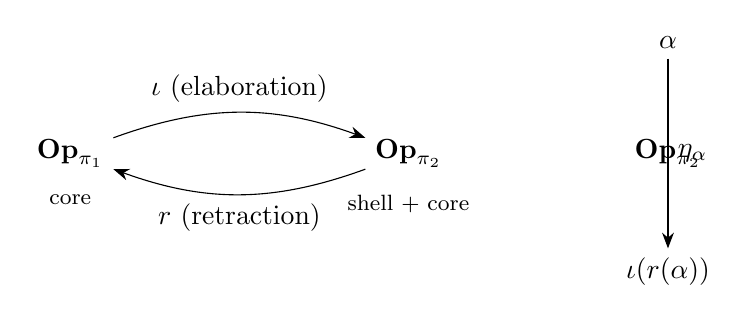
\begin{tikzpicture}[
  node distance = 24mm and 32mm,
  every node/.style = {align=center},
  >={Stealth[length=2mm]}
]
  \node (op1) {$\mathbf{Op}_{\pi_1}$};
  \node[right = of op1] (op2) {$\mathbf{Op}_{\pi_2}$};
  \draw[->,bend left=20] (op1) to node[above]{$\iota$ (elaboration)} (op2);
  \draw[->,bend left=20] (op2) to node[below]{$r$ (retraction)} (op1);
  \node[right = 22mm of op2] (op2b) {$\mathbf{Op}_{\pi_2}$};
  \node[above = 9mm of op2b] (etaa) {$\alpha$};
  \node[below = 9mm of op2b] (etab) {$\iota(r(\alpha))$};
  \draw[->] (etaa) -- node[right]{$\eta_\alpha$} (etab);
  \node[below = 1mm of op1] {\footnotesize core};
  \node[below = 1mm of op2] {\footnotesize shell + core};
\end{tikzpicture}
\caption{The elaboration adjunction $r \dashv \iota$ between the
$\pi_1$-coherent core operad and the $\pi_2$-coherent
shell-plus-core operad. The unit $\eta_\alpha$ exhibits each
shell-strategy $\alpha$ as a canonical extension of its retracted
core $r(\alpha)$.}
\label{fig:lx-adjunction}
\end{figure}

\section{Examples}

We illustrate the elaboration adjunction structure on two empirical cases that
the broader project has already worked through informally.

\begin{example}[Rearranging-to-Make-Bases LX to Counting-On]
Let $\pi_1$ correspond to the vocabulary of plain counting (Counting
On, CO): the operations of repeated successor and predecessor on
integers, no base-alignment shortcut. Let $\pi_2$ extend this with
the vocabulary of base-aligned moves (Rearranging-to-Make-Bases, RMB):
$\mathrm{delta\_to\_next\_base}_b$, base-aligned $\mathrm{iter\_succ}$
with reduced cost. We claim:
\begin{itemize}[noitemsep,topsep=2pt]
  \item $\iota$ embeds every CO program as an RMB program with no
        base-alignment shortcut activated.
  \item $r$ retracts every RMB program to the CO program obtained by
        replacing each base-aligned $\mathrm{iter\_succ}$ chunk with
        its expansion as repeated unit successor.
  \item $r \circ \iota$ is the identity: a CO program elaborated to
        RMB without using the shortcut, then retracted, returns the
        original CO program.
  \item The unit $\eta_\alpha : \alpha \to \iota(r(\alpha))$, for an
        RMB program $\alpha$, displays $\alpha$ as a particular
        re-organisation of the underlying CO program — the explicit
        articulation of the base-aligned structure that was tacit in
        CO.
\end{itemize}
This matches the empirical claim that RMB stands LX to CO: it makes
the associative property and the utility of base boundaries explicit,
where CO only used them implicitly.
\end{example}

\begin{example}[Fractional Composition Scheme LX to Partitive
Fractional Scheme]\label{ex:fcs}
Let $\pi_1$ be the vocabulary of partitive fraction operations
(PFS): partition, disembed, iterate, with the result of a single
PFS run as the output type. Let $\pi_2$ extend this with the
vocabulary of recursive partitioning: the operation
$\mathrm{accommodate}$ that re-assigns the output of one PFS run as
the input ``Whole'' for the next, plus the resulting Fractional
Composition Scheme (FCS) as a strategic shell.
\begin{itemize}[noitemsep,topsep=2pt]
  \item $\iota$ sends every PFS operation to its image as a
        single-level FCS (no recursion engaged).
  \item $r$ retracts every FCS operation to the PFS computation
        obtained by ``flattening'' the recursive substitution,
        reducing the strategic shell to its inner partition.
  \item The unit $\eta_\alpha$, for an FCS operation $\alpha$,
        displays $\alpha$ as an operadic substitution: the shell
        invokes PFS as a subroutine at the recursive slot. This is
        precisely the ``metamorphic accommodation'' described in
        \textcite{steffeOlive2010, hackenberg2007} formalised
        operadically.
\end{itemize}
The example is canonical: it is the case in which the empirical
project has already articulated the LX-relation in operational
detail. The categorical refinement says nothing the empirical work
did not already imply; what it does is make the structure portable
and composable.
\end{example}

\section{The fractal architecture as iterated LX}

The empirical project has documented an elaboration chain across
arithmetic strategies:
\[
\mathrm{CO} \;\to\; \mathrm{RMB} \;\to\; \mathrm{Chunking} \;\to\;
\mathrm{Skip\ Counting} \;\to\; \mathrm{C2C} \;\to\;
\mathrm{Distributive\ Reasoning} \;\to\; \mathrm{CGOB\ Division}
\]
with each arrow representing an algorithmic elaboration in which
prior practice is taken up as a callable subroutine. In the
operadic-LX framework this chain is a sequence of elaboration adjunctions
\[
r_1 \dashv \iota_1,\quad r_2 \dashv \iota_2,\quad \dots,\quad
r_k \dashv \iota_k
\]
between successively richer sub-operads. Adjunctions compose:
$(r_2 r_1) \dashv (\iota_1 \iota_2)$. The full elaboration chain is a
single adjunction between the smallest operad in the chain
(plain counting) and the largest (the most-elaborated strategy
catalogue), with intermediate vertices given by the partial
compositions.

\begin{proposition}[LX-towers compose]
\label{prop:tower}
Given elaboration adjunctions $r_i \dashv \iota_i$ for $i = 1, \dots, k$, the
composition $r_k \cdots r_1 \dashv \iota_1 \cdots \iota_k$ is an
elaboration adjunction between the head and tail of the chain.
\end{proposition}

\begin{proof}
Composition of adjoint pairs is an adjoint pair; the elaboration and
retraction conditions are preserved component-wise.
\end{proof}

\begin{corollary}[Fractal self-similarity is operadic substitution]
The empirical observation that arithmetic strategies are
``self-similar'' — that strategies at one level invoke strategies at
prior levels as subroutines — is formally captured by operadic
substitution at LX-extended sub-operads. The unit of the composed
elaboration adjunction, evaluated on a high-level strategy, displays the
entire chain of subordinate strategies as nested explicit content.
\end{corollary}

This is the structural reading of the empirical ``fractal
architecture'': not a metaphor of self-similarity, but a precise
statement that strategies form a tower of elaboration adjunctions whose units
exhibit the operadic substitution structure.

\section{Open problems and a deferred question}\label{sec:open}

The framework as stated raises several questions.

\begin{enumerate}[noitemsep,topsep=2pt,label=(\arabic*)]
  \item \textbf{Existence and uniqueness of $r$.} Definition~\ref{def:lx}
        posits an adjoint pair without giving construction rules for
        $r$. For arithmetic strategies the retraction is usually
        evident — strip the shell, expose the core — but a general
        criterion under which $r$ exists, and is unique up to
        natural isomorphism, would convert the definition into a
        theorem.
  \item \textbf{Descent along the metaphor cover.} The metaphor
        cover is closed under substitution within a label
        (Prop.~\ref{prop:cover-closure}) but not across labels.
        Documented strategy bridges that cross metaphors — for
        example the rotation-by-$180^\circ$ blend that joins
        Object Collection to Motion Along a Path for integer
        multiplication — should correspond to descent data along
        the cover. Whether the metaphor cover satisfies a
        Grothendieck-topology condition strong enough to admit
        descent is open.
  \item \textbf{Limits of LX-towers.} Proposition~\ref{prop:tower}
        gives finite composition. What is the colimit of an infinite
        ascending tower of elaboration adjunctions? In Brandomian terms: what
        does it mean to take the limit of an ascending chain of
        elaborated-explicating practices? Is the colimit the
        ``conceptual closure'' of arithmetic — and if so, is it
        well-defined?
  \item \textbf{Multi-base LX.} The base-shift functor of the
        companion paper preserves cost when cost is structural. Does
        it also preserve elaboration adjunctions? If a strategy stands LX to
        its core in base $10$, does its base-shifted image stand LX
        to the base-shifted core in base $12$?
  \item \textbf{Algebraic computation of explicitness.} The unit
        $\eta_\alpha$ of an elaboration adjunction supplies the explicit
        content of a strategy. Can $\eta_\alpha$ be computed
        algebraically from $\alpha$, $\iota$, and $r$ — for example,
        as a derived operation in the operad? An affirmative answer
        would give us a procedure for ``reading the explicit content
        off'' any elaborated strategy, which would be
        pedagogically and computationally useful.
\end{enumerate}

\paragraph{A deferred question.} A natural further question is
whether LX is self-applicable: whether a vocabulary $V$ can stand
LX to itself. The Brandomian intuition is that a vocabulary that
makes its own implicit features explicit constitutes a kind of
reflective closure. The categorical question is whether a self-LX
functor — an endo-adjunction of the form $r \dashv \iota$ with
$r \circ \iota = \mathrm{id}$ on some sub-operad and $\iota \circ r
\ne \mathrm{id}$ on the whole — admits fixed points or
diagonalisation phenomena analogous to those of self-referential
formal systems. This question connects to the broader project's
work on the More Machine and on Gaifman's reading of G\"odel's
incompleteness theorems. We do not pursue it here; it is genuinely
interesting but tangential to the structural results of the
present note.

\section{Conclusion}

The operadic refinement and the elaboration adjunction proposal are the same
move read in two registers. Operadic substitution is the operation
along which adjunctions compose; LX is the conceptual interpretation
of substitution as elaboration with an explicitness witness. Together
they make the empirical project's ``fractal architecture'' — strategies
built as strategic shells around iterative cores, in towers — a
precise categorical structure. The elaboration adjunction is portable: any
domain in which practices are elaborated from prior practices and
make explicit what was tacit admits the same analysis, given an
operadic presentation of its primitives.

The framework is not a theory of cognition. It is a categorical
proposal: that LX, treated as an adjunction with computable unit,
gives a working formalisation of what mathematics-education researchers
call ``conceptual understanding''. The empirical project's existing
work on twenty-five arithmetic strategies — the iterative-core /
strategic-shell pattern, the substitution-based nesting, the
elaboration chains across operation families — populates the structure
with concrete examples. What remains is to either prove or disprove
the adjointness condition in each case, and to ask whether the open
questions of \S\ref{sec:open} have meaningful answers.

\printbibliography

\end{document}
